\documentclass[11pt,letterpaper,onecolumn]{article}
\usepackage[english]{babel}
\usepackage[compact]{titlesec}
\usepackage[titles]{tocloft}
\usepackage[super]{cite}
\usepackage{%
  float,
  amssymb,
  amsmath,
  fullpage,
  textcomp,
  gensymb,
  hyperref,
  listings,
  caption,
  sectsty,
  bm,
  times,
  empheq,
  booktabs
}
\usepackage[framed,numbered,autolinebreaks,useliterate]{../sty/mcode}

\newcommand{\figurepath}{../fig/term-project}
\newcommand{\codepath}{../include/code/term-project}

\setlength{\parindent}{0.0in}

%------------------------------------------------------------------------
% Section
\makeatletter
 \renewcommand\section{\@startsection{section}{1}{\z@}%
 {-3.5ex \@plus-1ex \@minus-0.2ex}%
 {1.0ex \@plus0.2ex}%
 {\fontsize{12pt}{12pt}\selectfont\bfseries\sffamily}}
 \makeatother
% Subsection
\makeatletter
 \renewcommand\subsection{\@startsection{subsection}{1}{\z@}%
 {-3.5ex \@plus-1ex \@minus-0.2ex}%
 {0.5ex \@plus0.2ex}%
 {\fontsize{10pt}{10pt}\selectfont\bfseries\sffamily}}
 \makeatother
% Subsubsection
\makeatletter
 \renewcommand\subsubsection{\@startsection{subsubsection}{1}{\z@}%
 {-3.5ex \@plus-1ex \@minus-0.2ex}%
 {0.5ex \@plus0.2ex}%
 {\fontsize{10pt}{10pt}\selectfont\bfseries}}
 \makeatother
%------------------------------------------------------------------------

%------------------------------------------------------------------------
\setlength\cftparskip{-3pt}
\setlength\cftbeforesecskip{1pt}
\setlength\cftaftertoctitleskip{1pt}
\cftsetindents{figure}{0em}{1.5em}
\makeatletter
\renewcommand{\@dotsep}{4.5}
\renewcommand{\cftdotsep}{4.5}
\renewcommand{\cftsecdotsep}{4.5}
\renewcommand{\@tocrmarg}{4.55em}
\makeatother
\renewcommand\cftsecfont{\normalfont}
\renewcommand\cftsecpagefont{\normalfont}
\renewcommand{\cftsecleader}{\cftdotfill{\cftsecdotsep}}
%------------------------------------------------------------------------

\def\listofsymbols{\begin{tabbing}
  % YOU NEED TO ADD THE FIRST ONE MANUALLY TO ADJUST THE TABBING AND SPACES
  $x$~~~~~~~~\=\parbox{5in}{Position (east)}\\
  %ADD THE REST OF SYMBOLS WITH THE HELP OF MACRO
  \addsymbol y: {Position (north)}{symbol:y}
  \addsymbol z: {Altitude}{symbol:z}
  \addsymbol V: {Total airspeed}{symbol:V}
  \addsymbol \gamma: {Flight path angle}{symbol:gamma}
  \addsymbol \psi: {Heading angle (measured clockwise from north, or positive $y$-axis)}{symbol:psi} 
  \addsymbol \phi: {Roll angle}{symbol:phi}
  \addsymbol p: {Roll rate}{symbol:p}
  \addsymbol m: {Mass}{symbol:m}
  \addsymbol \rho: {Density}{symbol:rho}
  \addsymbol C_{L}: {Lift coefficient}{symbol:CL}
  \addsymbol C_{D}: {Drag coefficient}{symbol:CD}
  \addsymbol C_{D_{0}}: {Parasitic drag coefficient}{symbol:CD0}
  \addsymbol S: {Wing area}{symbol:S}
  \addsymbol E_{\text{max}}: {Best lift-to-drag-ratio}{symbol:Emax}
  \addsymbol L: {Lift}{symbol:L}
  \addsymbol D: {Drag}{symbol:D}
  \addsymbol k: {Induced drag factor}{symbol:k}
  \addsymbol W_{x}: {Horizontal wind velocity}{symbol:Wx}
  % ALWAYS KEEP THE FOLLOWING LINE
\end{tabbing}
}
\def\addsymbol#1: #2#3{$#1$ \> \parbox{5in}{#2}\\}
\def\newnot#1{\label{#1}}

\title{Optimal Dynamic Soaring of an Albatross}
\author{
Daniel P. Wiese\thanks{Graduate Student, Mechanical Engineering, 77 Massachusetts Avenue Rm 3--441} \\
{\normalsize\itshape{}Massachusetts Institute of Technology, Cambridge, MA 02139, USA} \\[4pt]
}

\begin{document}

\begin{titlepage}
  \begin{center}
    \rule{\linewidth}{0.01in} \\[0.25in]
    { \huge \bfseries Optimal Dynamic Soaring of an Albatross }\\[0.4cm]
    \rule{\linewidth}{0.01in} \\[0.25in]

    \textsc{\LARGE Term Project Spring 2014 }\\[0.05in]
    \textsc{\Large 16.323 Optimal Control}\\[0.25in]
    \large Due: Tuesday, May 6, 2014 \\[1.1in]
    
\includegraphics[width=1.5in]{../fig/mit-seal.pdf}\\[2.9in]
    % Author and instructor
    \begin{minipage}{0.4\textwidth}
      \begin{flushleft} \large
        \emph{Author:}\\
        Daniel \textsc{Wiese}
        \vfill
      \end{flushleft}
    \end{minipage}
    \begin{minipage}{0.4\textwidth}
      \begin{flushright} \large
        \emph{Instructor:} \\
        Prof.~Steven \textsc{Hall} \\
      \end{flushright}
    \end{minipage} \\
    \vfill
  \end{center}
\end{titlepage}

\clearpage

\begin{abstract}
  \textbf{
    This work presents an analysis and comparison of an optimal control solution for the dynamic soaring of an albatross with experimental data.
    Three different wind profiles were examined, and the problem of interest was maximizing the upwind progress an albatross could make during periodic, or traveling dynamic soaring.
    Representative geometrical and aerodynamic properties of a typical wandering albatross were gathered from the literature to use in the numerical simulation, where the solver GPOPS was used to obtain the optimal trajectory.
    This optimal solution when a linear, logarithmic, or power-law horizontal wind profile was used was compared to GPS data.
    The relevant data such as average groundspeed, peak altitude, and average cycle time were compared and agreed to well within one order of magnitude.
    It was determined that the albatross make forward progress into the wind with groundspeed approximately equal to the wind velocity.
    The trajectory verified the following dynamic soaring rule: climb into the wind, descend away from the wind.
    These solutions were found to be very sensitive to the wind gradient near the surface, as well as the lower altitude constraint limit.
  }
\end{abstract}

\section{List of Symbols}

\listofsymbols%

\section{Introduction and Problem Statement}

Soaring is defined as sustained flight which does not require external thrust.
\textit{Dynamic soaring} is a term used more specifically when the flight involves energy extraction from horizontal wind, as opposed to vertical wind components.
It was first suggested by Lord Rayleigh in 1883 that birds may take advantage of dynamic soaring, and a substantial amount of research has been conducted since then.\cite{rayleigh.soaring.1883} We now understand that birds such as the wandering albatross have evolved to leverage this phenomenon, allowing them to make flights which last around 10 days, flying more than 1000 km per day.
The information gained from learning about how the wandering albatross utilizes dynamic soaring could be used to develop bio-inspired UAVs designed for long distance travel.
Such UAVs could have applications in surveillance, search and rescue, and environmental monitoring, staying aloft for weeks at a time and covering thousands of miles with minimal energy consumption\cite{richardson.highspeedrobotic.2012}.

\subsection{The Wandering Albatross}

The wandering Albatross is a large sea bird with 3.5 meter wing span, the largest of the animal kingdom.
It has a special bone structure which allows it to ``lock-in'' its wings to the fixed, outstretched position without requiring the use of its muscles to flap its wings or hold them in place while flying.
This means that the albatross maintains its flying configuration with essentially zero energy expenditure.
It has an aspect ratio of about 16, and weighs between 7--10 kg.
Some noteworthy figures are the range of the best lift-to-drag ratio of between 18--27\cite{barnes.howflies.2004,alexander.naturesflyers.2004,denny.dynamicsoaring.2009} and maximum lift coefficient of 1.15--1.5\cite{pennycuick.glidingpetrel.1960,wood.flight.1973,pennycuick.flight.1982}.
The relevant quantities are listed in Table~\ref{tab.albatrossdata}.
This data was based on representative data~\cite{tucker.falconaero.1970,wood.flight.1973,pennycuick.flight.1982} as compiled in Reference [\citen{sachs.minimumshear.2005}].

\begin{figure}[h]
  \begin{center}
    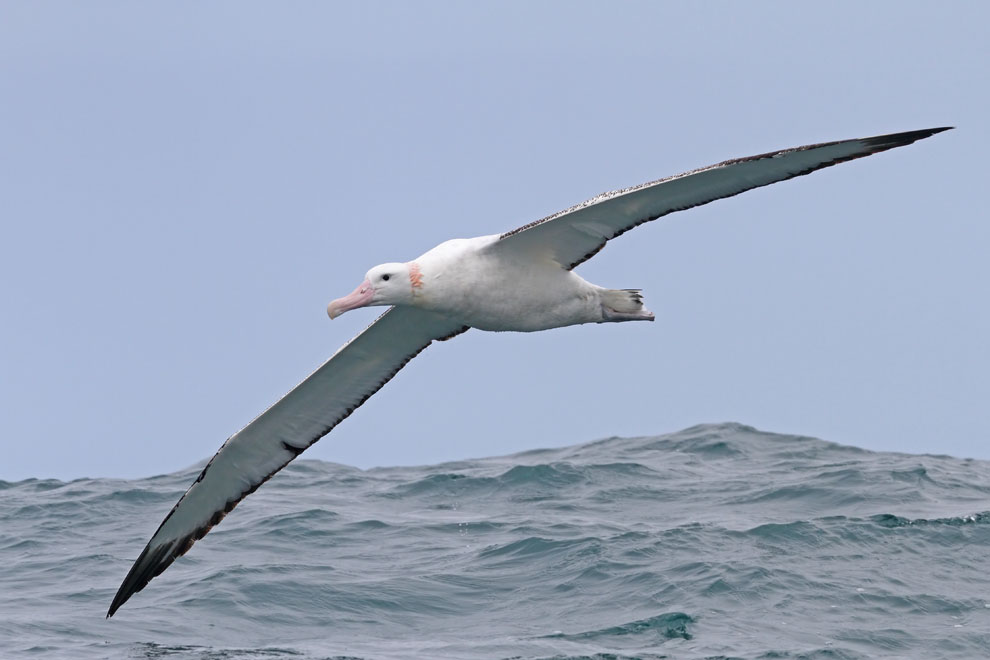
\includegraphics[width=2.6in]{\figurepath/albatross.jpg}
    \caption{The wandering albatross. \url{http://www.stephenburch.com/}\label{fig:part3_multiple_state}}
  \end{center}
\end{figure}

\begin{table}[H]
  \centering
  \caption{Albatross properties}
  \begin{tabular}{lcrc}
    \toprule
    Parameter                   & Symbol              & Value   & Unit \\ \midrule
    Mass                        & $m$                 & $8.5$   & kg \\
    Wing area                   & $S$                 & $0.65$  & m$^{2}$ \\
    Wingspan                    & $b$                 & $3.44$  & m \\
    Parasitic drag coefficient  & $C_{D_{0}}$         & 0.033   & --- \\
    Maximum lift coefficient    & $C_{L,\text{max}}$  & 1.5     & --- \\
    Best lift-to-drag ratio     & $E_{\text{max}}$    & 20      & --- \\
    \bottomrule
  \end{tabular}\label{tab.albatrossdata}
\end{table}

\subsection{Problem Statement}\label{sec.problemstatement}

The problem that was considered in this work is stated as follows: Given a typical boundary layer profile that might be observed over a flat field or calm sea, determine the optimal trajectory for an albatross to fly to maximize its distance travelled into the wind.

In Section~\ref{sec.eom} we provide the equations of motion which describe the albatross during dynamic soaring, and discuss the wind profile model used, the state constraints that must be satisfied while the albatross is soaring, and the assumptions that were made in deriving the model.
In Section~\ref{sec.optimalproblem} we formulate the problem as an optimal control problem, and discuss how the solver GPOPS was used to numerically determine a solution.
In Section~\ref{sec.results} we present the results of the numerical solution, and provide a discussion and interpretation of these results.

\section{Equations of Motion}\label{sec.eom}

The anatomy of the albatross and its ability to keep its wings stretched makes it behave essentially like a fixed-wing glider, with some differences which will be discussed later.
The equations of motion describing the albatross are the following\cite{zhao.optimalpatterns.2004}

\begin{equation}
  \begin{split}\label{eqn.eom}
    \dot{x}       &= V\cos\gamma\sin\psi+W_{x} \\
    \dot{y}       &= V\cos\gamma\cos\psi \\
    \dot{z}       &= V\sin\gamma \\
    \dot{V}       &= -\frac{1}{m}D-g\sin\gamma-\dot{W}_{x}\cos\gamma\sin\psi \\
    \dot{\gamma}  &= \frac{\cos\phi}{mV}L-\frac{1}{V}g\cos\gamma+\frac{1}{V}\dot{W}_{x}\sin\gamma\sin\psi \\
    \dot{\psi}    &= \frac{\sin\phi}{mV\cos\gamma}L-\frac{\cos\psi}{V\cos\gamma}\dot{W}_{x} \\
    \dot{\phi}    &= p \\
    \dot{C}_{L}   &= -bC_{L}+bC_{L,\text{cmd}}
  \end{split}
\end{equation}

where $x$ is the position corresponding to east, $y$ is north, $V$ is the airspeed, $\gamma$ is the flight path angle, $\psi$ is the heading angle, $\phi$ is the roll angle, and $p$ is the roll rate.
$L$ and $D$ are the lift and drag, and $W_{x}(z)$ and $\dot{W}_{x}(z)$ define the wind profile, and time rate of change in the wind experienced by the albatross during flight.
The lift and drag are given by the following well-known equations

\begin{align}
  L &=\frac{1}{2}\rho V^{2}SC_{L} \\
  D &=\frac{1}{2}\rho V^{2}SC_{D}
\end{align}

where $\rho$ is the density of air, $S$ is the planform area, and $C_{L}$ and $C_{D}$ are the lift and drag coefficients, respectively.
The total drag coefficient is calculated as follows

\begin{equation}
  C_{D}=C_{D_{0}}+kC_{L}^{2}
\end{equation}

where $C_{D_{0}}$ is the parasitic drag coefficient, and $k$ is the induced drag factor.
The induced drag factor can be calculated as

\begin{equation}
  k=\frac{1}{4E_{\text{max}}^{2}C_{D_{0}}}
\end{equation}

where $E_{\text{max}}$ is the maximum lift-to-drag ratio, given as

\begin{equation}
  E_{\text{max}}=\left(\frac{C_{L}}{C_{D}}\right)_{\text{max}}
  =\left(\frac{C_{L}}{C_{D_{0}}+kC_{L}^{2}}\right)_{\text{max}}
\end{equation}

The inputs to this system of equations is the roll rate $p$ and the commanded lift coefficient $C_{L,\text{cmd}}$.
The lift coefficient was included as a state in~\eqref{eqn.eom} to capture the dynamics which govern the ability of the albatross to change its lift during flight.
During dynamic soaring, it can be advantageous to abruptly change the lift generated, but with outstretched wings there is a finite rate at which the albatross can do this.
By effectively filtering the lift coefficient as an input it required changes in the albatrosses lift coefficient to be smooth, as would be expected during flight.
For the same reason the roll rate was used as an input instead of the roll angle.

\subsection{State-Space Formulation}

The system of equations in~\eqref{eqn.eom} can be represented as

\begin{equation*}
  \dot{X}=f(X,U)
\end{equation*}

where the state vector $X$ and input $U$ are given by

\begin{equation*}
  \begin{split}
    X &=
    \begin{bmatrix}
      x & y & z & V & \gamma & \psi & \phi & C_{L}
    \end{bmatrix} \\
    U &=
    \begin{bmatrix}
      C_{L,\text{cmd}} & p
    \end{bmatrix}
  \end{split}
\end{equation*}

This is the representation of the dynamic constraint which will be inputed into the solver to obtain the optimal trajectory as discussed in the following section.

\subsection{Wind Profile}

The essence of dynamic soaring is the extraction of energy from a horizontal wind-shear gradient.
Such a gradient is necessary for dynamic soaring, and so the particulars of the wind profile are of great importance.
This gradient is strong within an altitude of about 20 meters above the surface, after which the wind speed remains essentially constant.
The wind profile is accurately modeled using the following logarithmic function\cite{cone.mathematical.1964,wood.flight.1973,pennycuick.flight.1982}

\begin{equation*}
  \mbox{\textbf{Logarithmic}}
  \hspace{0.5in}
  W_{x}(z)=W_{x,\text{ref}}\frac{\ln(z/z_{0})}{\ln(z_{\text{ref}}/z_{0})}
\end{equation*}

with derivative

\begin{equation*}
  \frac{dW_{x}}{dz}=\frac{W_{x}}{\ln(z_{\text{ref}}/z)}\frac{1}{z+z_{0}}
\end{equation*}

A more convenient and less accurate of the wind profile is to use a linear model, given by

\begin{equation*}
  \mbox{\textbf{Linear}}
  \hspace{0.5in}
  W_{x}(z)=\frac{W_{x,\text{ref}}}{z_{\text{ref}}}z
\end{equation*}

with derivative

\begin{equation*}
  \frac{dW_{x}}{dz}=\frac{W_{x,\text{ref}}}{z_{\text{ref}}}
\end{equation*}

This linear model is less representative of the actual wind profile, but can be more convenient when evaluating the numerical solution.
Another wind model that is suggested is the power-law wind profile,\cite{barnes.howflies.2004} given below.
This model is often preferred over the linear profile because it is a more accurate representation of the actual wind profile.
It is often preferred over the logarithmic profile due to the fact that the logarithmic profile has an infinite gradient at the surface, and the wind velocity never actually diminishes with an increase in altitude, whereas the following power-law profile has a finite gradient at the surface and diminishes

\begin{equation*}
  \mbox{\textbf{Power-law}}
  \hspace{0.5in}
  W_{x}(z)=\frac{W_{x,\text{ref}}}{1-e^{-a}}\left(1-e^{-a\frac{z}{z_{\text{ref}}}}\right)
\end{equation*}

with derivative

\begin{equation*}
  \frac{dW_{x}}{dz}=\left(\frac{a}{z_{\text{ref}}}\right)\left(\frac{W_{x,\text{ref}}}{1-e^{-a}}\right)e^{-a\frac{z}{z_{\text{ref}}}}
\end{equation*}

The time derivative $\dot{W}_{x}$ is evaluated using the chain rule as

\begin{equation*}
  \dot{W}_{x}=\frac{dW_{x}}{dt}=\frac{dW_{x}}{dz}\frac{dz}{dt}=\frac{dW_{x}}{dz}V\sin\gamma
\end{equation*}

Each of these three wind profiles is plotted in Figure~\ref{fig.windplot} below.

\begin{figure}[h]
  \begin{center}
    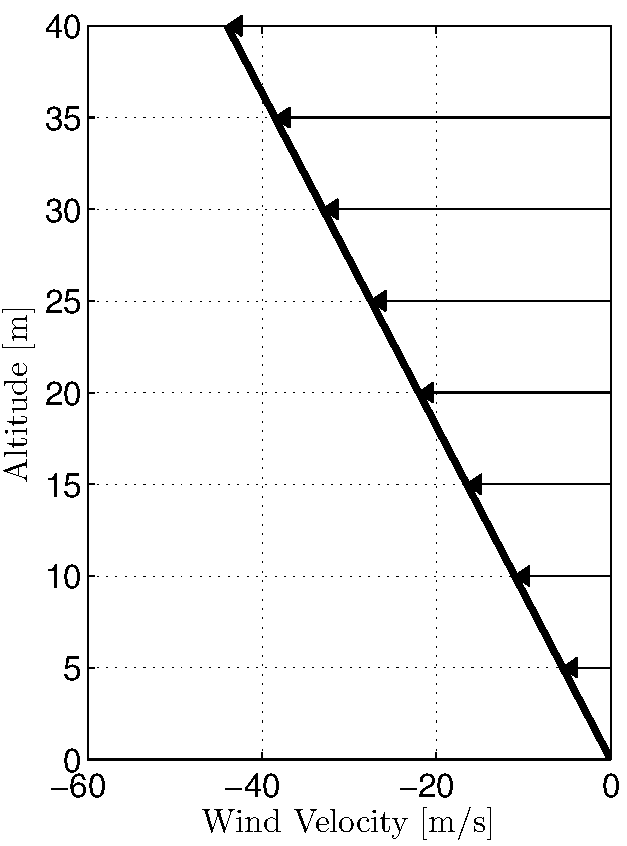
\includegraphics[height=2.2in]{\figurepath/plot_wind_lin.pdf}
    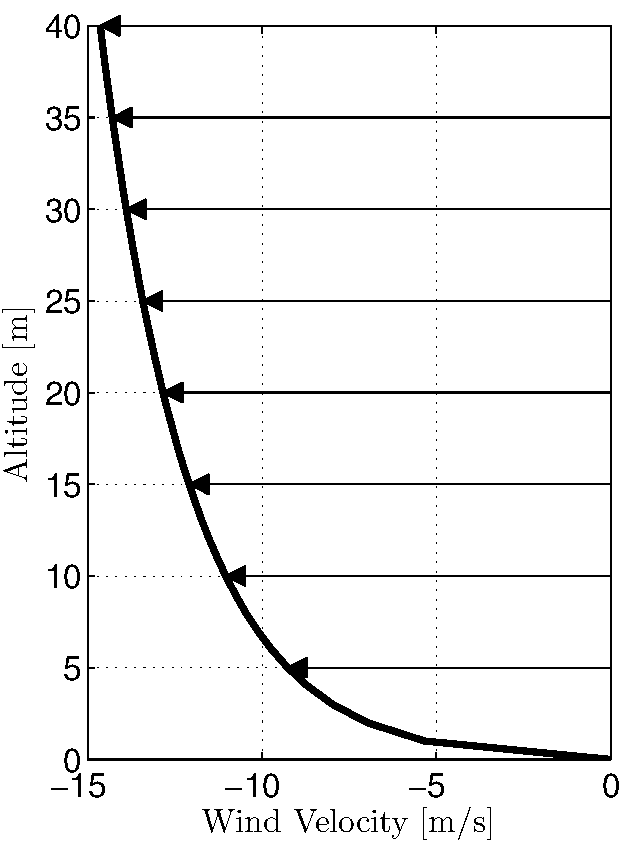
\includegraphics[height=2.2in]{\figurepath/plot_wind_log.pdf}
    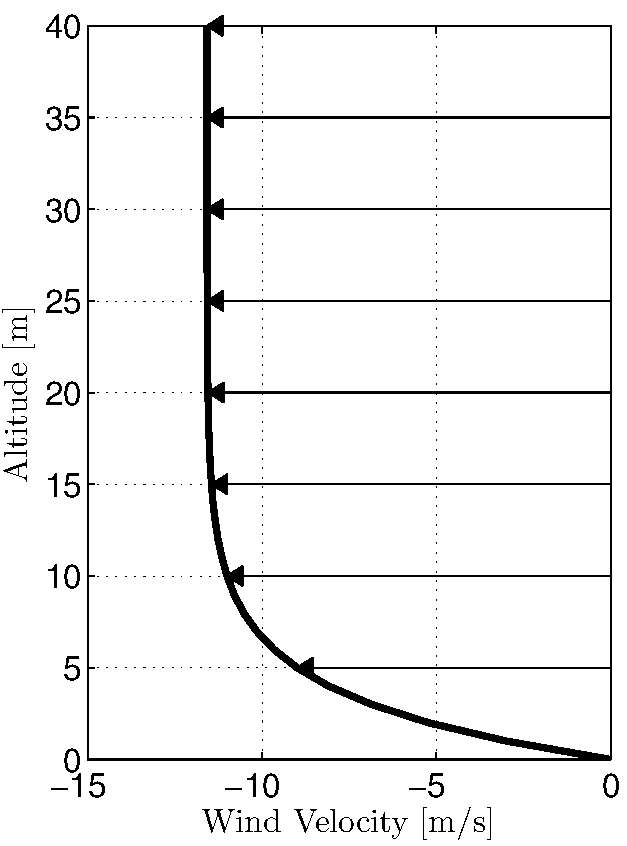
\includegraphics[height=2.2in]{\figurepath/plot_wind_exp.pdf}
    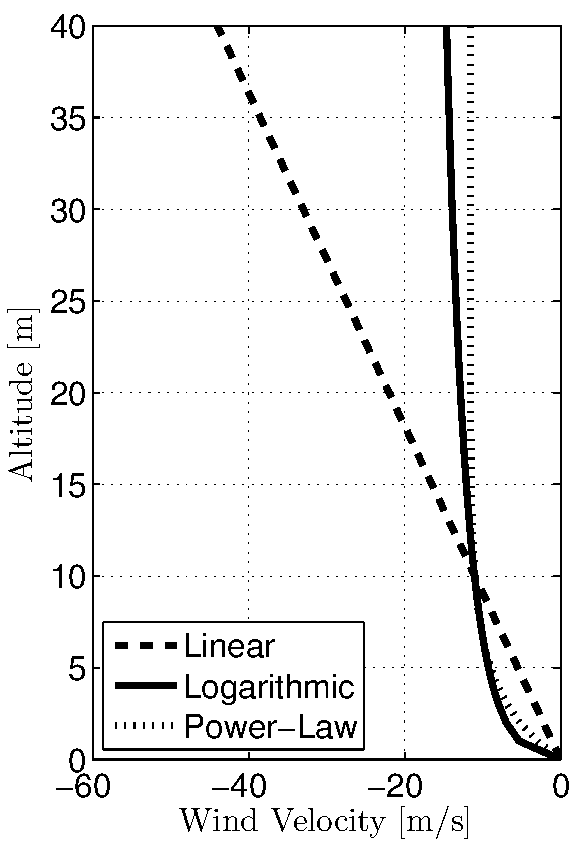
\includegraphics[height=2.2in]{\figurepath/plot_wind_linlog.pdf}
    \caption{Plot of the wind over the surface for linear, logarithmic, and power-law profiles, from left to right. The fourth figure shows a comparison between each velocity profile.\label{fig.windplot}}
  \end{center}
\end{figure}

\subsection{State Constraints}\label{subsec.stateconstraints}

In nearly any optimal control problem, there will exist constraints on the state, both at the initial and terminal times, as well as along the trajectory.
To obtain an optimal control solution which resembles experimental data, it is important to accurately capture what the state constraints are that an albatross must satisfy during soaring flight.

During dynamic soaring, that is without flapping its wings, $v_{\text{min}}=12$ m/s, is the minimum airspeed that the bird requires to maintain lift\cite{wilson.sweeping.1975,videler.avianflightbook.2005}.
There is not much of a practical upper limit on airspeed\cite{catry.sustainedfast.2004} but observed data suggests $v_{\text{max}}=47$ m/s is a reasonable upper limit.
Observed bank angles are estimated to be in the range 55--70 degrees.\cite{idrac.experimentelle.1932,pennycuick.gust.2002} No data could be found on observed flight path angle limits for albatrosses.
Because the wind gradient provides the energy for dynamic soaring, and because the wind will have a gradient which is largest at the surface, the minimum altitude at which the albatross flies greatly impacts its ability to use dynamic soaring.
Observations have shown that it is not uncommon for the wingtips of the albatross to skim the water when soaring.
A lower limit of 1 meter was selected as the minimum altitude.
A peak altitude of between 8--30 meters has been observed during typical soaring.
40 meters was selected as the upper limit.

%\subsection{Model Assumptions}
%
%One of the primary differences between a bird such as the albatross and a conventional glider, is the birds ability to actively adjust parameters such as camber, twist, and taper during flight, unlike a glider.

\section{Optimal Control Problem Formulation}\label{sec.optimalproblem}

In terms of an optimal control problem formulation, the problem statement in Section~\ref{sec.problemstatement} is stated as: determine the optimal control inputs $C_{L,\text{cmd}}$ and $p$ to minimize the following objective function, subject to the state dynamics, initial, terminal and path constraints.
The objective function is given by

\begin{equation*}
  \min_{C_{L,\text{cmd}},p}J=-x(t_{f})
\end{equation*}

indicating the desired objective is to maximize the distance travelled upwind.
The boundary conditions are given as

\begin{equation*}
  \begin{split}
    x(t_{0})  &= 0 \\
    y(t_{0})  &= 0 \\
    z(t_{0})  &= 10 \\
    V(t_{0})  &= 24
  \end{split}
\end{equation*}

with the following conditions used to enforce periodicity of the flight path for what is called \textit{traveling dynamic soaring}.
That is, the albatross should complete a dynamic soaring maneuver repetitively to make forward progress into the wind.

\begin{equation*}
  \begin{split}
    z(t_{0})      &= z(t_{f}) \\
    V(t_{0})      &= V(t_{f}) \\
    \gamma(t_{0}) &= \gamma(t_{f}) \\
    \psi(t_{0})   &= \psi(t_{f}) \\
    \phi(t_{0})   &= \phi(t_{f}) \\
    C_{L}(t_{0})  &= C_{L}(t_{f})
  \end{split}
\end{equation*}

The path constraints are given by the following, where these values are representative of the observed data discussed in Section~\ref{subsec.stateconstraints}.

\begin{equation*}
  \begin{split}
    1\leq     & z \\
    12\leq    & V\leq47 \\
    -75\leq   & \gamma\leq75 \\
    -80\leq   & \phi\leq80 \\
    -1.5\leq  & C_{L}\leq1.5
  \end{split}
\end{equation*}

where the altitude is expressed in [m], the velocity is expressed in [m/s], and the angles expressed in [deg].
In determining the optimal solution, the following numerical values were used for the wind profile.

\begin{table}[H]
  \centering
  \caption{Environment properties}
  \begin{tabular}{lcrc}
    \toprule
    Parameter                   & Symbol              & Value   & Unit \\ \midrule
    Air density                 & $\rho$              & $1.225$ & kg/m$^{3}$ \\
    Reference windspeed         & $W_{x,\text{max}}$  & -11     & m/s \\
    Reference altitude          & $z_{\text{ref}}$    & 10      & m \\
    Logarithmic wind parameter  & $z_{0}$             & 0.15    & m \\
    Power-law wind parameter    & $a$                 & 3       & --- \\
    \bottomrule
  \end{tabular}\label{tab.environmentdata}
\end{table}

\subsection{Solution Method}

After the optimal control problem was formulated, the solver GPOPS was used to numerically determine a solution to the dynamic soaring problem for the three different wind profiles described above.
GPOPS uses collocation, which approximates trajectories using Lagrange interpolating polynomials to essentially represent the problem as a constrained function optimization problem, or nonlinear program.
This is known as a transcription method.
Once the problem has been cast as a nonlinear program, GPOPS has different NLP solvers which can be used.

\section{Results and Discussion}\label{sec.results}

Figures~\ref{fig.xyzplot_lin}-\ref{fig.xyzplot_exp} show the trajectory of the albatross as it attempts to maximize its distance traveled in the positive $x$-direction against the wind for the three different wind profiles.
The albatross starts the flight at the green circle, ending at the red x.
Analysis of these profiles verifies the following rule, known as the dynamic soaring rule.
Simply stated, this rule says to maximize dynamic soaring energy the albatross should climb into the wind and descend away from the wind.

\begin{figure}[H]
  \begin{center}
    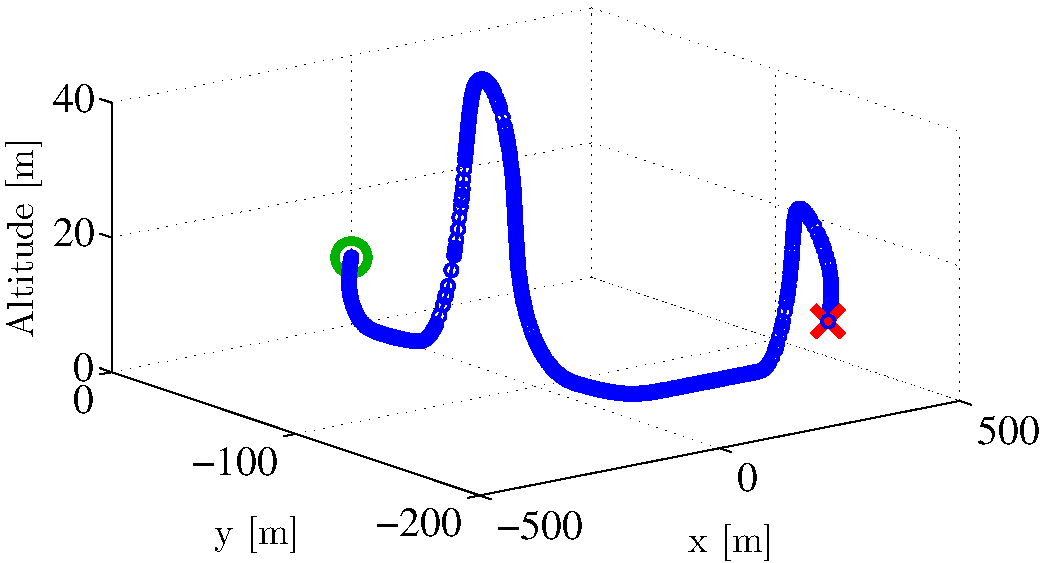
\includegraphics[width=3.0in]{\figurepath/plot_xyz_lin.pdf}
    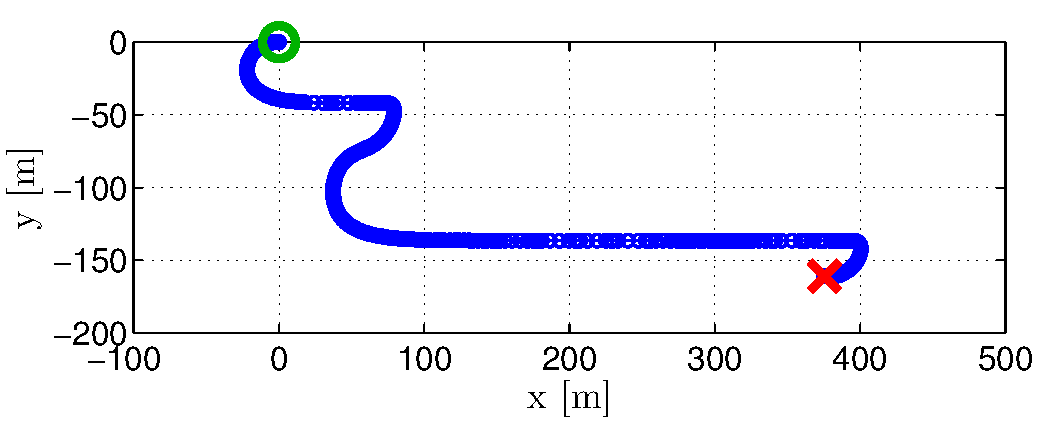
\includegraphics[width=3.0in]{\figurepath/plot_xy_lin.pdf}
    \caption{Optimal dynamic soaring trajectory of the albatross in the linear wind profile with $W_{x,\text{ref}}=-11$ m/s and $z_{\text{ref}}=10$ m.\label{fig.xyzplot_lin}}
  \end{center}
\end{figure}

\begin{figure}[H]
  \begin{center}
    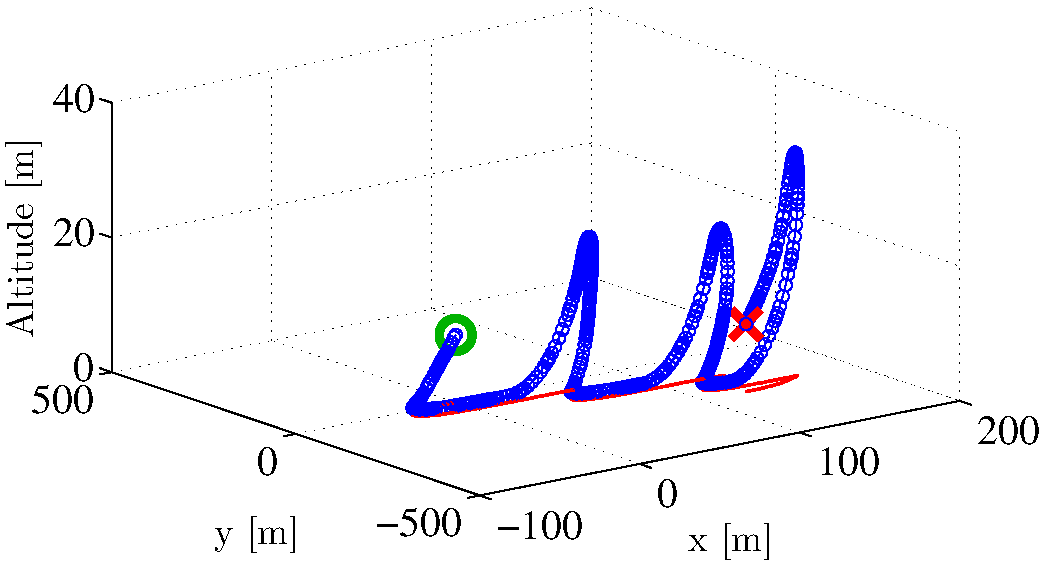
\includegraphics[width=3.5in]{\figurepath/plot_xyz_log.pdf}
    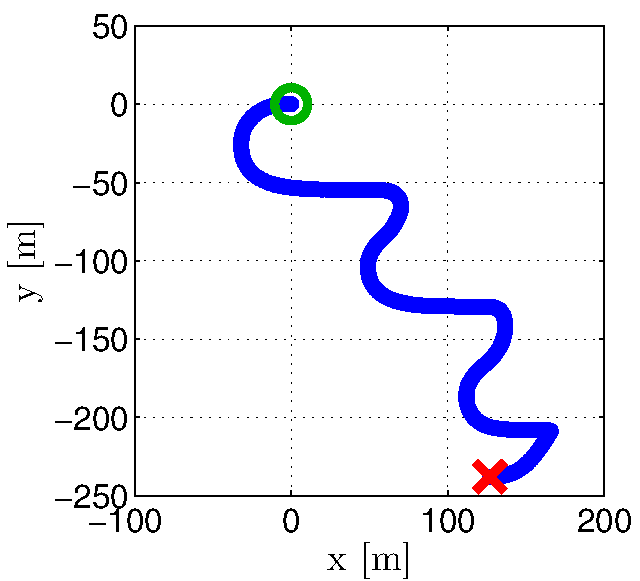
\includegraphics[width=2.5in]{\figurepath/plot_xy_log.pdf}
    \caption{Optimal dynamic soaring trajectory of the albatross in the logarithmic wind profile with $W_{x,\text{ref}}=-11$ m/s, $z_{\text{ref}}=10$ m, and $z_{0}=0.15$ m.\label{fig.xyzplot_log}}
  \end{center}
\end{figure}

\begin{figure}[H]
  \begin{center}
    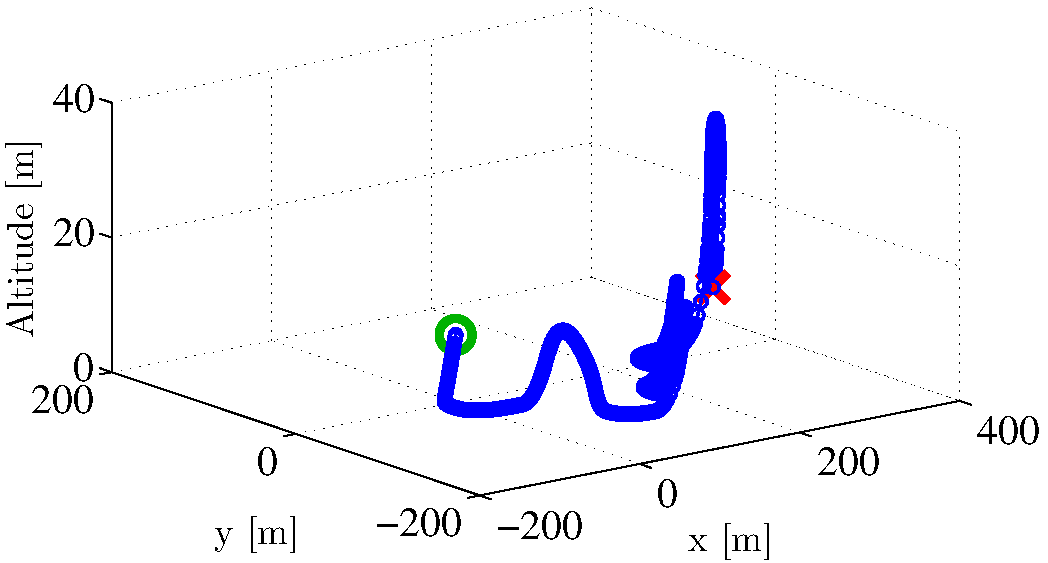
\includegraphics[width=3.0in]{\figurepath/plot_xyz_exp.pdf}
    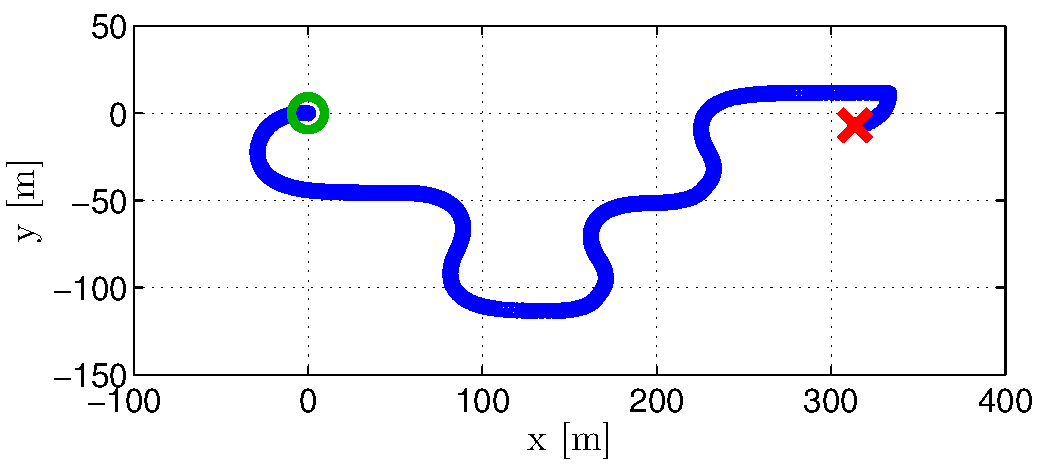
\includegraphics[width=3.0in]{\figurepath/plot_xy_exp.pdf}
    \caption{Optimal dynamic soaring trajectory of the albatross in the power-law wind profile with $W_{x,\text{ref}}=-11$ m/s, $z_{\text{ref}}=10$ m, and $a=3$.\label{fig.xyzplot_exp}}
  \end{center}
\end{figure}

\subsection{Comparison to Experimental Data}

The results of the dynamic soaring optimization described above were compared to some recently obtained data obtained for the flight of albatrosses equipped with a GPS sensor to monitor their flight path.
It has been reported in many observations that the typical dynamic soaring cycle is around 10 seconds, with peak altitudes of around 15 m being fairly common during moderate 10 m/s winds when the albatross is flying upwind.
Furthermore, upwind progress was observed to be between 4.6--7.6 m/s, depending on the strength of the wind.
These observations were verified by some recently obtained GPS data which captured several days worth of dynamic soaring data of an albatross.\cite{sachs.progress.2011,sachs.experimental.2013} This GPS data is consistent with the results obtained in the optimization, well within one order of magnitude of all the relevant quantities such as average groundspeed, peak altitude, and cycle time.
The relevant data for the optimization is collected in Table~\ref{tab.results} below.

\begin{table}[H]
  \centering
  \caption{Optimization results for different wind profiles when flying upwind}
  \begin{tabular}{lcccc}
    \toprule
    Wind Profile  & Average groundspeed [m/s] & Average Airspeed [m/s]  & Peak altitude [m] & Cycle time [s] \\ \midrule
    Linear        & 12.5                      & 25.7                    & 40.0              & 15.0 \\
    Logarithmic   & 5.4                       & 24.3                    & 29.5              & 7.5 \\
    Power-Law     & 10.5                      & 26.0                    & 34.0              & 7.5 \\ \midrule
    GPS data      & 6.1                       & 12.7                    & 9.8               & 7.5 \\
    \bottomrule
  \end{tabular}\label{tab.results}
\end{table}

It was found that the solution was highly dependent on the wind profile and the lower altitude constraint limit.
This is expected, as the velocity gradient is the mechanism through which the albatross extracts energy from the wind, and the gradient becomes increasingly large very near the surface.
Changing the wind profile parameters $a$ and $z_{0}$ very slightly resulted in relatively large differences in the solution.
Changing the lower altitude limit an order of 0.1 meters also had a noticeable impact on the solution.
Furthermore, the solution was sensitive to the constraints on roll angle and roll rate as well.
The more aggressively the albatross maneuvers, the more efficiently it can use dynamic soaring.
However, while gliders can be made to sustain g-loads of 30 or more, the albatross cannot tolerate more than about 3.
While the results overall matched well, it is noted that the power-law and logarithmic profiles are still a significant simplification of the profile that is experienced by an albatross flying over the ocean.
Waves greatly change the wind profile near the surface, causing eddies between wave crests, and updrafts of around 2 m/s.

\section{Conclusions and Future Work}

The optimal dynamic soaring trajectory for an albatross which maximizes distance traveled into the wind was determined using optimal control.
Using representative data describing the mass, geometry, and aerodynamic characteristics of an albatross, as well as a simplified wind model, the optimal trajectory is fairly close to GPS data taken from real albatrosses while performing dynamic soaring.
However, there are several major limitations that must be considered when comparing the optimal control solution to GPS data.
The first limitation is that the simplified wind profile model neglects wind eddies between wave crests, and the significant updrafts which are often present on the ocean.
Second, the GPS data which is recorded does not provide information about even the average wind during the flight of an albatross.
Lastly, the optimal control solution is very sensitive to small changes in the wind profile and the lower constraint limit on altitude, and so solutions can differ noticeably for small changes in these values.
This can make it hard to obtain an accurate optimal control solution and fairly compare it with the GPS data.
However, even with these limitations the optimal control solution for all three wind profiles is still a decent representation of the soaring observed in albatrosses.

In order to improve the optimal control solution and more accurately compare it with experimental data, it would be beneficial to improve the wind model.
To do this, more information should be compiled to determine a good representation of the average waves and wind profile on the open ocean on an average day.
Then, more GPS data should be collected with additional information gathered about the local wind speed near the albatross as it flies.

\bibliography{../bib/term-project.bib}
\bibliographystyle{aiaa}

\clearpage
\section{Appendix: Optimal Trajectory Plots}

\subsection{Linear Wind Profile}

\begin{figure}[H]
  \begin{center}
    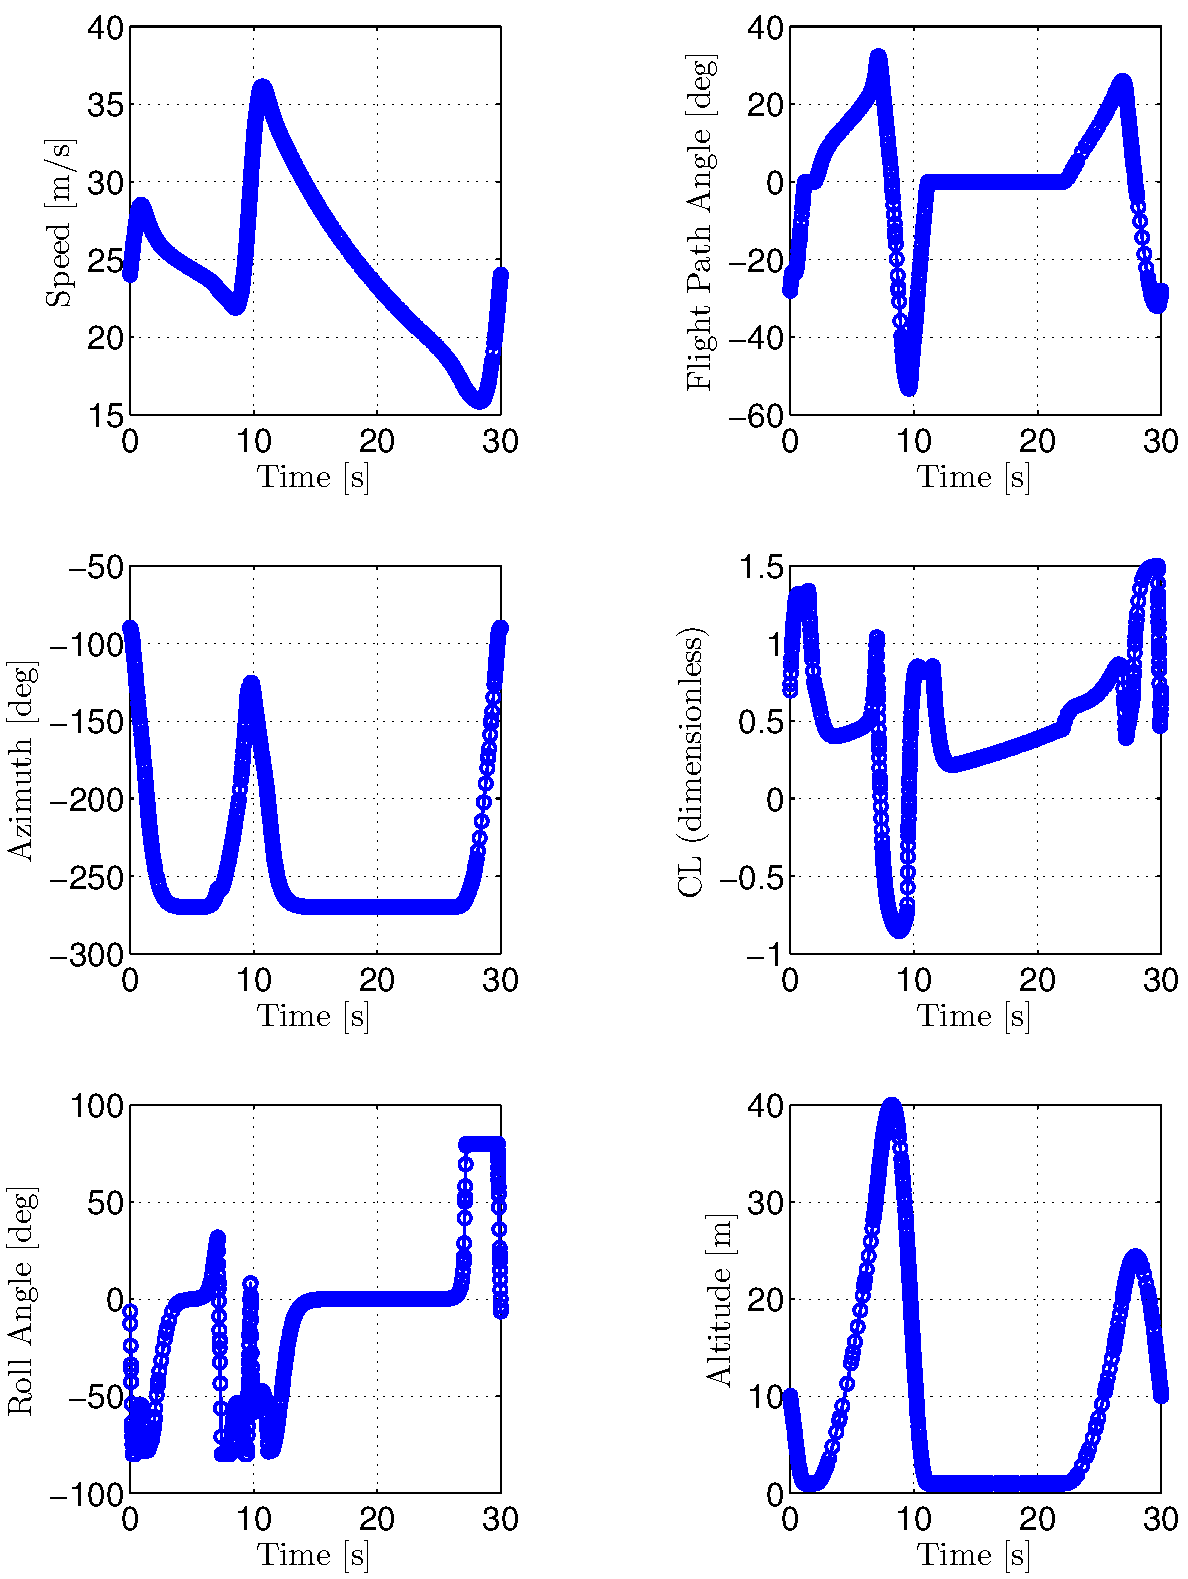
\includegraphics[width=5.0in]{\figurepath/plot_versus_t_lin.pdf}
    \caption{optimal dynamic soaring trajectory\label{fig.tplot_lin}}
  \end{center}
\end{figure}

\begin{figure}[H]
  \begin{center}
    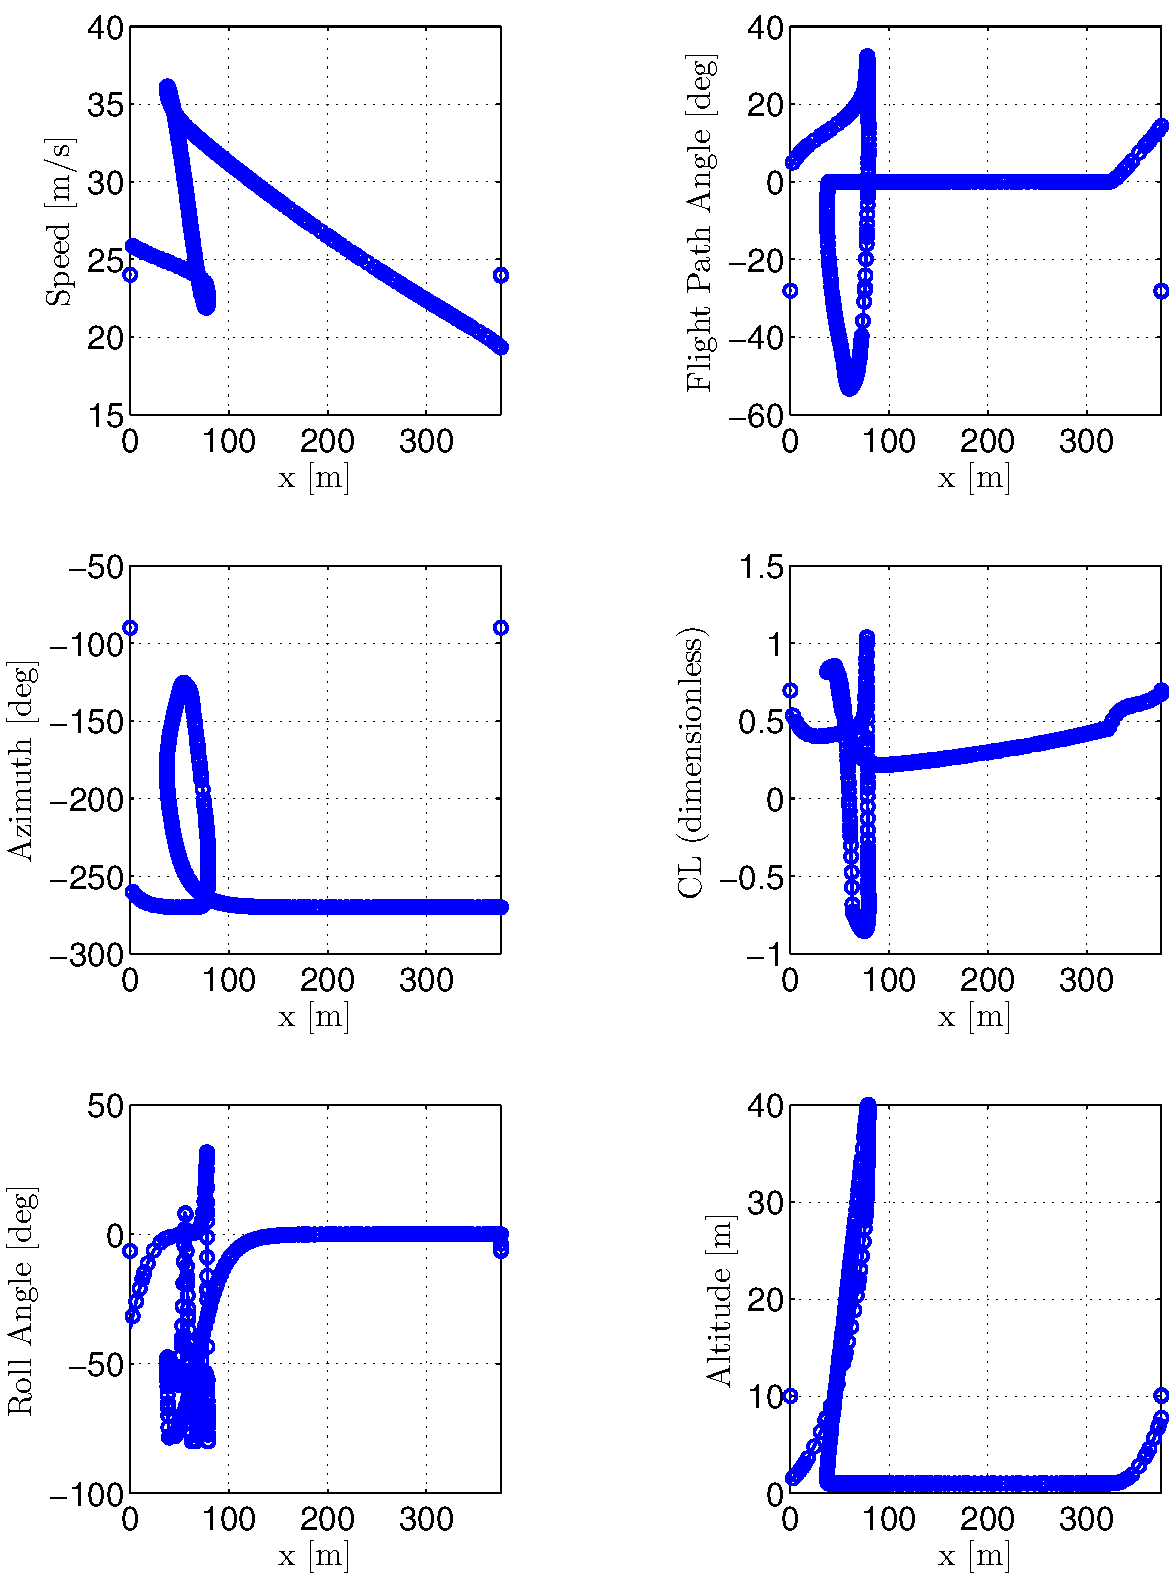
\includegraphics[width=5.0in]{\figurepath/plot_versus_x_lin.pdf}
    \caption{optimal dynamic soaring trajectory\label{fig.xplot_lin}}
  \end{center}
\end{figure}

\subsection{Logarithmic Wind Profile}

\begin{figure}[H]
  \begin{center}
    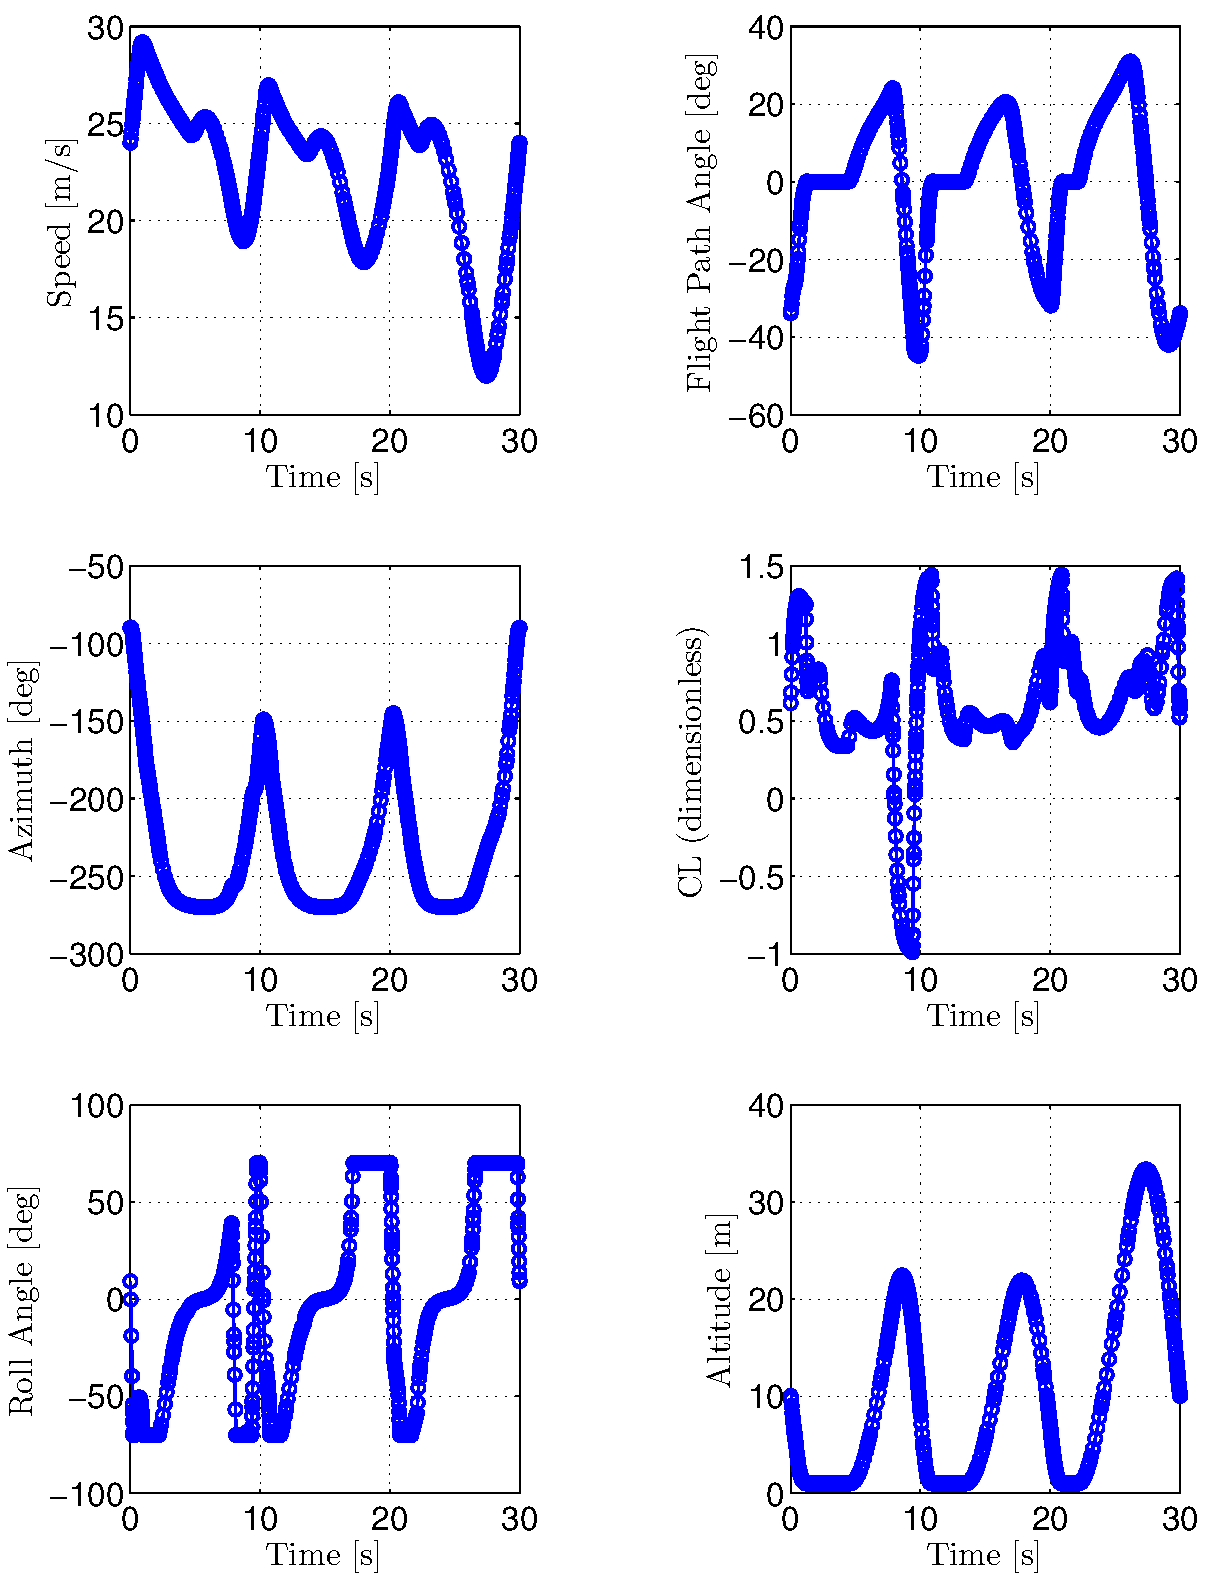
\includegraphics[width=5.0in]{\figurepath/plot_versus_t_log.pdf}
    \caption{optimal dynamic soaring trajectory\label{fig.tplot_log}}
  \end{center}
\end{figure}

\begin{figure}[H]
  \begin{center}
    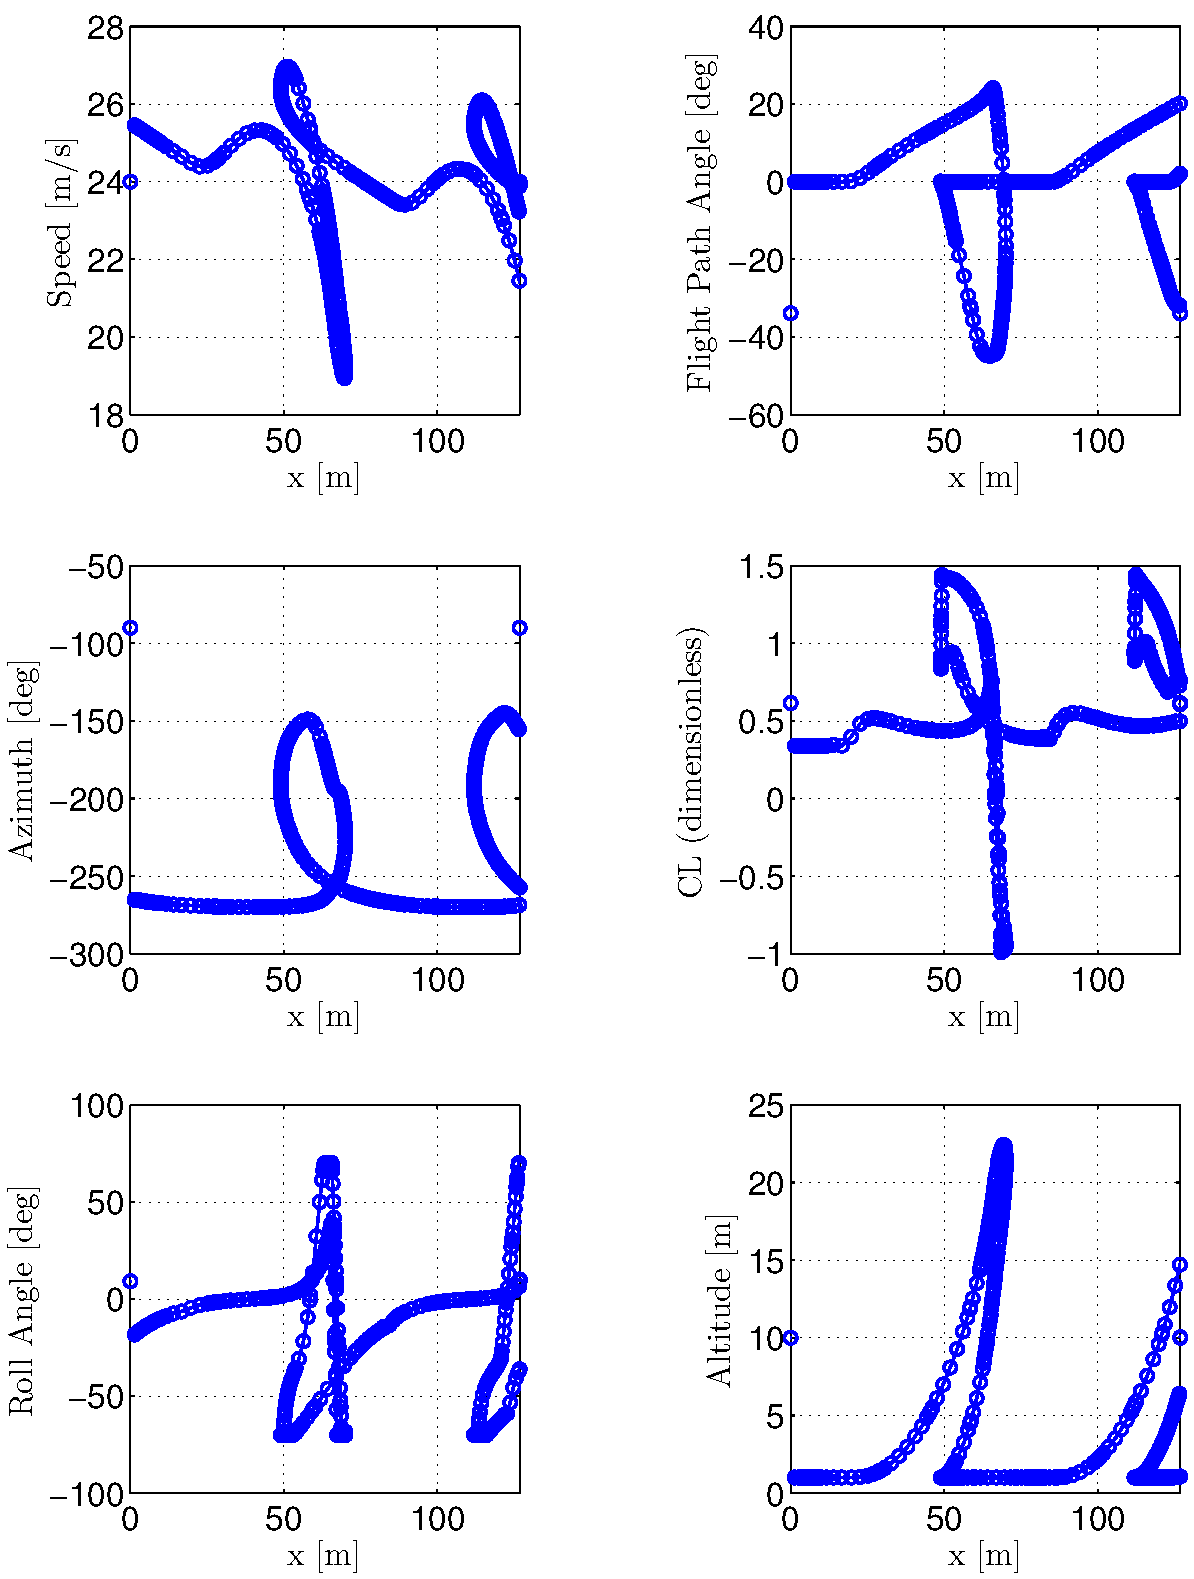
\includegraphics[width=5.0in]{\figurepath/plot_versus_x_log.pdf}
    \caption{optimal dynamic soaring trajectory\label{fig.xplot_log}}
  \end{center}
\end{figure}

\subsection{Power-Law Wind Profile}

\begin{figure}[H]
  \begin{center}
    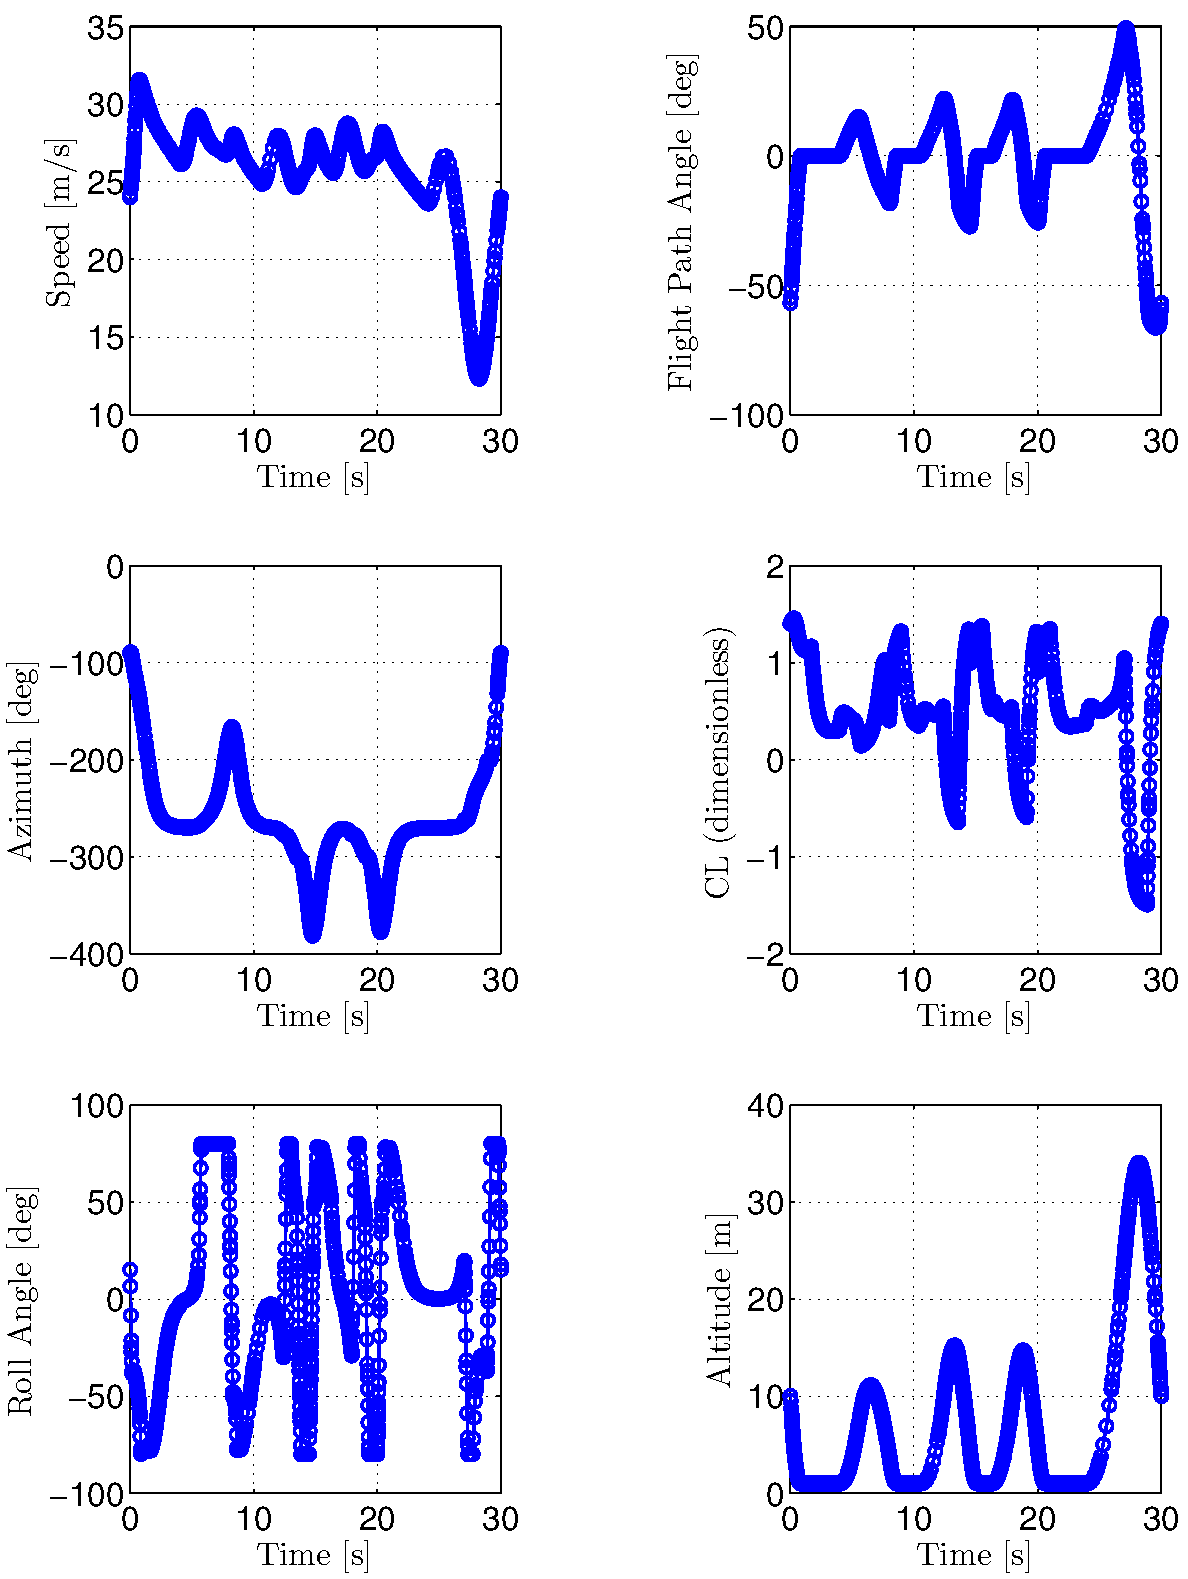
\includegraphics[width=5.0in]{\figurepath/plot_versus_t_exp.pdf}
    \caption{optimal dynamic soaring trajectory\label{fig.tplot_exp}}
  \end{center}
\end{figure}

\begin{figure}[H]
  \begin{center}
    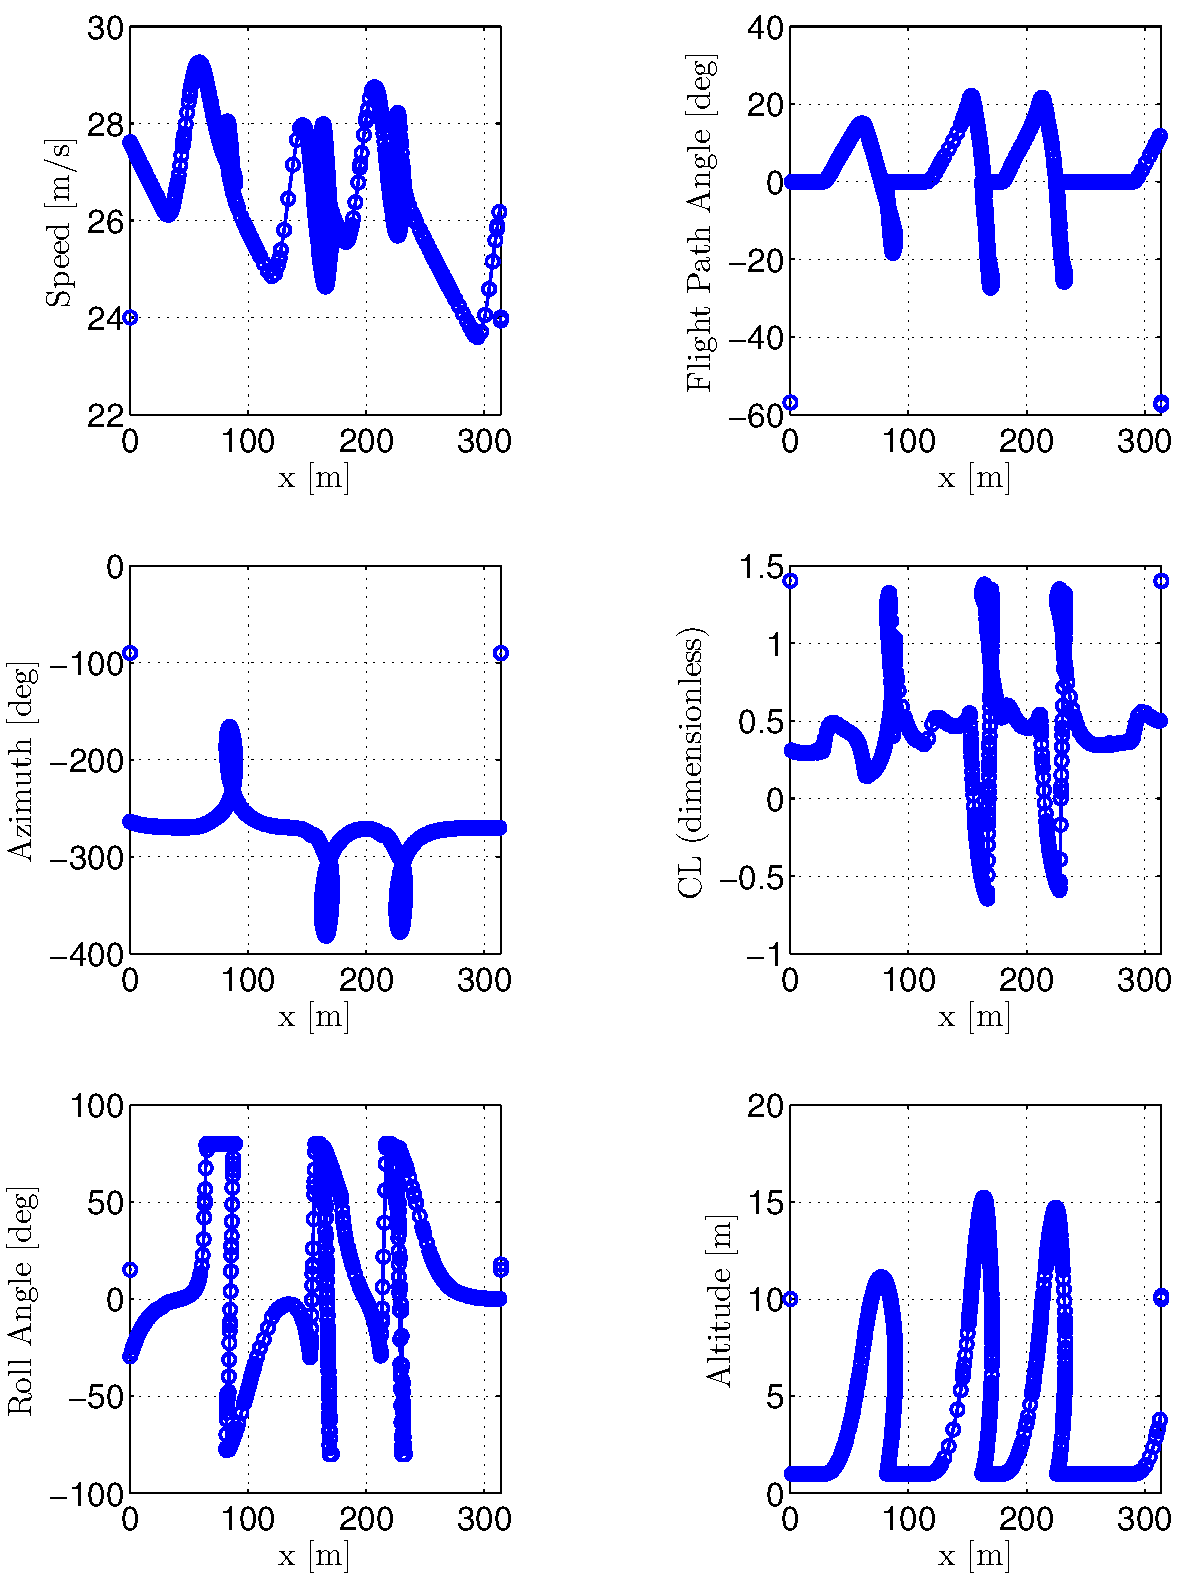
\includegraphics[width=5.0in]{\figurepath/plot_versus_x_exp.pdf}
    \caption{optimal dynamic soaring trajectory\label{fig.xplot_exp}}
  \end{center}
\end{figure}

\clearpage
\section{Appendix: Code}

\lstinputlisting{\codepath/dS_Main.m}
\lstinputlisting{\codepath/dS_Continuous.m}
\lstinputlisting{\codepath/dS_Endpoint.m}
\lstinputlisting{\codepath/dS_LoadGuess.m}
\lstinputlisting{\codepath/dS_PlotWind.m}
\lstinputlisting{\codepath/dS_Plotter.m}
\lstinputlisting{\codepath/dS_FileNamer.m}
\lstinputlisting{\codepath/dS_MakeMovie.m}

\end{document}
